\chapter{Dynamics of the gene expression machinery during an acetate-glucose upshift}
\chaptermark{Gene expr. machinery during an upshift}
\label{chap:experiments}

%\textit{"If reality does not fit the concept, too bad for reality."} -- Georg Wilhelm Friedrich Hegel

\selectlanguage{french}
\section*{Résumé en français du Chapître \thechapter : Dynamique de la machinerie d'expression génique lors d'une transition acétate vers glucose.}

Résumé d'environ 6-8 paragraphes (2 pages).
\selectlanguage{english}

\section{Introduction}

Most studies on the growth of microorganisms are done at steady state.
It is a reasonable and logical choice given the drawbacks of working in dynamic.
At steady state, microorganism behaviors are reproducible, and which helps uncover simple theories to apprehend their inherent complexity.
But while this ideal environment is easily achievable at the bench, microorganisms naturally spend very little time in such a perfect condition.
This motivated in chapter~\ref{chap:theory} the construction of a new theoretical framework to study growth laws during growth transitions.

The principles that define the regulatory processes in dynamic appear to be different than the ones that apply at steady state.
We showed that efficient regulatory strategies have to be able to perform extremely abrupt and intense variations of the gene activity.
This relies on the fact that bang-bang synthesis of gene expression machinery settles the upper-bound for biomass production during an environmental change.
Such strategies are only implementable if the regulatory system focus on the internal state of the cell.
But not all information is equivalent, and performing a near-perfect transition might require to measure several variables, a concept totally missing from steady-state considerations.
Interestingly, we uncovered how the ppGpp regulatory system of \textit{E. coli} might be a cheap way for the cell to access just enough information, and to implement a \textit{on-off} strategy to regulate the synthesis of ribosomes.
Overall, it taught us that the actual complexity of regulatory systems is only beneficial in a dynamical context.
But elucidating what is the best behavior, and showing that \textit{E. coli} actually implement it are different matters...

Reality actually highlights the problem with adopting a dynamical perspective on growth.
There are far more information on ribosome abundance at steady state than during growth transitions.
It is widely admitted that the latter are hard to control and rely too much on hidden variables about the strain history~[citation ? Bremmer ?].
Though, as we discussed in section~\ref{sec:discussion}, some data are available and seem to confirm that during growth transitions, the  synthesis rate of ribomoses can oscillate~\cite{gausing_regulation_1980,zengel_transcription_1986}, and that the ppGpp regulatory system can go through rapid changes~\cite{friesen_synthesis_1975,murray_control_2003}.
But we cannot decisively validate or disprove the model predictions from measurements that were carried out at the population level, where it is inherently hard to identify switching patterns.
What we need are dynamical single-cell measurements of the ribosome concentration during well-controlled growth transitions.
Would the \textit{on-off} strategy be observed, it could confirm the importance of optimizing transitions for the organism.
Would it be disproved, that could raise even more interesting questions: growth rate and biomass might not necessarily be what natural selection care for, or other unexpected limitations might prevent the cell to behave optimally.

In Chapter~\ref{chap:theory}, we developed a model of resource allocation during growth transitions.
By applying optimal control theory, we predicted that in order to maximize biomass production, the cell should produce its gene expression machinery in a bang-bang manner.
The full model with dimensional parameters is reproduced below, with dotted variables representing their time derivative:
\begin{eqnarray}
\dot{p}(t) &=& e_M(t)\cdot (1/\beta - r(t)) - \frac{k_R \cdot p(t)}{K_R + p(t)}\cdot r(t) \, (1+\beta\, p(t)), \label{eq:pdef-exp}\\
\dot{r}(t) &=& \frac{k_R \cdot p(t)}{K_R + p(t)}\cdot r(t) \, (\alpha(t) - \beta\, r(t)). \label{eq:rdef-exp}
\end{eqnarray}
In this form, it contains 4 variables ($e_M(t)$, $p(t)$, $r(t)$, $\alpha (t)$) and 3 parameters ($\beta$, $k_R$, $K_R$).
$e_M(t)$ [min\textsuperscript{-1}] is the richness of the environment.
$p(t)$ [g.L\textsuperscript{-1}] is the precursor concentration inside the cell.
$r(t)$ [g.L\textsuperscript{-1}] is the gene expression machinery concentration inside the cell.
$\alpha (t)$ [$\emptyset$] is the mass ratio of resources that goes to the gene expression machinery.
$k_R$ [min\textsuperscript{-1}] is the rate constant of macromolecular synthesis.
$K_R$ [g.L\textsuperscript{-1}] is the half-saturation constant of macromolecular synthesis.
$\beta$ [L.g\textsuperscript{-1}] is the inverse of the cellular density of macromolecules (assumed constant).
The goal of this chapter is to measure in vivo $\alpha (\cdot)$ during a growth transition, and check how it compares with the gold standard established in chapter~\ref{chap:theory}.

To this end, we took the challenge of measuring ribosomal abundance of \textit{E. coli} at the single-cell level during a controlled upshift.
We made a strain displaying fluorescent ribosomes, thus allowing in-vivo measurement of their abundance in dynamical conditions.
We placed it in a microfluidic device allowing the long-term imaging of individual cells while they are presented different growing media, and focused on the classic upshift from acetate to glucose.
We then used Kalman smoothing to estimate the variations of the growth rate and the relative ribosomal synthesis rate during this upshift.
While not allowing a decisive validation of the expected behavior, this experiment opens interesting questions and is a step towards a better understanding of the gene expression machinery regulation during growth transitions.

\section{Results}

\subsection{Experimental design}
\label{sec:exp_design}

How does one measure resource allocation in real cells?
There is no direct way to measure $\alpha (\cdot)$ in an experiment, mostly because of its abstract nature.
To correctly reconstruct it, one has to know the value of every single term in the equations in which it appears.
In the full dynamical system Eqs~\ref{eq:pdef-exp}-\ref{eq:rdef-exp}, $\alpha$ only pops up in Eq.~\ref{eq:rdef-exp}, and is already isolated in this equation, which simplifies the burden.
We can identify $\alpha (t_k)$ for each time $t_k$ where the following 3 terms are known: $\beta r(t_k)$, $\dot{r}(t_k)$, and $\frac{k_R \cdot p(t_k)}{K_R + p(t_k)} \cdot r(t_k)$.
Such a consideration remains valid if one can estimate the 6 individual components $r(t_k)$, $\dot{r}(t_k)$, $p(t_k)$, $k_R$, $K_R$, $\beta$.
Even if we assume that the constant parameters are known, or at least easier to estimate independently, reconstructing the dynamics of $\alpha$ would require to co-estimate the gene expression machinery concentration ($r$, $\dot{r}$) and the precursor concentration $p$.

Are such measurements acceptable?
Measuring the abundance of gene expression is achievable if one focus on a proxy that represents the overall abundance.
Ribosomes are widely known to be the most abundant part of the gene expression machinery, which allows to consider it as its main component~\cite{scott_interdependence_2010, scott_bacterial_2011,scott_emergence_2014}.
Their abundance can be estimated for instance by using the total RNA of the cell~\cite{scott_interdependence_2010}, radioactive markers\cite{gausing_regulation_1980,zengel_transcription_1986}, or fluorescent labeling~\cite{bakshi_superresolution_2012}.
Estimating precursor abundance is more challenging.
There is no clear proxy that represents all the precursors in the cell, so using common methods would be excessively time expensive~[citation classic methods to estimate precursor ?].
While absolute quantification of all the internal metabolites has been achieved in \textit{E. coli}~\cite{bennett_absolute_2009}, this method do not comply with our need of real-time single-cell quantification.

This problem can be overcome by using a simple transformation.
Taking into account that by construction the growth rate  $\mu(t)$ is given by:
\[
	\mu (t) = \beta \frac{k_R \cdot p(t)}{K_R + p(t)} \cdot r(t),
\]
we can rewrite Eq.~\ref{eq:rdef-exp} as follows
\begin{equation}
\label{eq:dot_r}
\dot{r}(t) = \mu (t) \, \left(\frac{\alpha(t)}{\beta} - r(t) \right).
\end{equation}
The problem of estimating $\alpha(\cdot)$ is thus equivalent to the same problem where $r(\cdot)$, $\dot{r}(\cdot)$, $\mu (\cdot)$ and $\beta$ have to be co-estimated.
If we are satisfied with estimating $\alpha$ up to a constant factor $\beta$, dynamically measuring the ribosome concentration and the growth rate would make $\alpha (\cdot) / \beta$ identifiable.

These new measurements are more acceptable given the requirements of the study.
We want to be able to identify potential abrupt changes of the gene expression.
Such switching patterns are easily hidden at the population level if cells are not synchronous, which is generally the case.
A short sample time and single-cell measurements are thus necessary, which motivated the use of fluorescent reporters like the green fluorescent protein (gfp).
We constructed a strain displaying a gfp-tagged S2 ribosomal subunit (the gene name being \textit{rpsB}).
The \textit{rpsB-gfp} strain produces fluorescent ribosomes, making them quantifiable while minimizing the burden for the cell (see Material and Methods~\ref{sec:methods_strain}).
By observing such a strain through a microscope during a growth transition, we could theoretically estimate the ribosome concentration by measuring the cell fluorescence, and reconstruct the growth rate by measuring the cell size.

The growth conditions might also play a role in the limitations of the study.
In natural conditions, the most straightforward growth transitions, or at least the one at which most of the selection is expected to occur, is the transition from the stationary phase in nutrient-deprived medium to any medium sustaining growth.
There are good reasons though for which this particular growth transition is ignored from most studies.
The transition from stationary to exponential phase is dramatically ill-controlled, in the sense that a lot of hard-to-control parameters seem to play a huge role in it.
For instance, this is the case of the duration of the nutritive stress~[citation to find], the nutrient encountered during the last exponential phase~[citation to find], or the previous accumulation of wastes in the medium~[citation to find].
This somehow results in a phenomenon called the lag phase~[citation lag phase review to find], the mechanisms of which are missing from our model.
Furthermore, most microorganisms dramatically change their physiology in stationary-phase, either sporulating or organizing into biofilms~[citations subtilis sporulation and coli biofilms to find], which goes largely beyond the scope of this study.
For this reason, we decided to focus on a transition from a slow exponential growth to high exponential growth, in particular the transition from acetate to glucose.
By construction, this steady-state-to-steady-state transition requires a long acquisition time before and after the shift, respectively to ensure cells have \textit{forgotten} the previous stress phase, and have enough time to reach the new steady state.
The mothermachine, a microfluidic device that was designed to sustain exponential growth for long period of time, seemed like a good choice for this purpose.
It allows to maintain a constant flow of fresh medium around the cells, and make fast transitions possibles by switching the medium that is fed to the cells (see Material and Methods~\ref{sec:growth_condition} and \ref{sec:microflu}).
The complete experimental scheme is summarized in Fig.~\ref{fig:experiment_schema}.

\begin{figure}[tb]
\centering
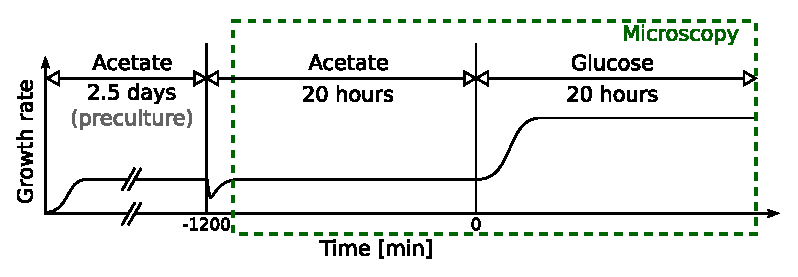
\includegraphics[scale=1]{./Fig/experiment_schema.eps}
\caption{
\textbf{Scheme of the upshift experiment.}
The goal is to measure the fluorescence and growth rate of cells during an acetate-to-glucose upshift.
All the media used are M9 minimal medium supplemented with 0.2\% of the indicated carbon source, in this case acetate or glucose (see Material and Methods~\ref{sec:growth_condition}).
The \textit{rpsB-gfp} strain was precultivated for 2.5 days on 0.2\% acetate in batch condition (shaken flask).
The day of the experiment, the cells were injected into the mothermachine and fed by a constant flow of fresh 0.2\% acetate medium (see Material and Methods~\ref{sec:microflu}).
Fluorescence and phase contrast images were taken every 5 minutes.
Twenty hours later, the feeding media was switched to 0.2\% glucose (known to theoretically sustain a 5-time-higher growth rate) and was maintained for twenty more hours while imaging carried on.
Time 0 corresponds to the exact moment when cells start to be in contact with the glucose medium.
}
\label{fig:experiment_schema}
\end{figure}

\subsection{Data acquisition}

It is important to evoke most of the issues that occurred while carrying on the experiment.
At the time, a serious issue was starting to affect our only microscope: the motorization along the Z-axis was randomly stalling until an operator manually intervenes.
This deactivates the autofocus and the Z-compensation for the tilt of the device when moving along the XY plane.
In other words, series of images are out of focus and thus not exploitable if the operator was not around, which can happen a lot in a 40-hour-long experiment.
For the experiment presented here, we timed the operations so that the operator can be around as long as possible when it counts, \textit{i.e.} close to the transition at time 0.
This is the reason why data points between -720 and -150 minutes are not available (corresponding to the steady state on acetate).
Another issue, more specific to the presented occurence of the experiment, was that bacteria started to massively die several hours after the transition.
The reason is unknown, the most plausible hypothesis being a phage contamination.
\footnote{Note that the operator was present when the dying started, which excludes the implication of lab gnomes.}
Data analysis was thus stopped at 550 minutes, when roughly 3/4 of the cells were still growing.
Note that for these reasons, the results of this preliminary experiment must be taken with caution.
The necessary improvements are extensively discussed in section~\ref{sec:chap3_discussion}.

Image analysis was performed on the remaining shots.
While image analysis softwares overflow the literature~[citations schitcells + others], some of them being specifically designed for the mother machine~[molysso + Wang et al], technical limitations did not allow to use any of them.
For instance, the segmentation was systematically impeded by the poor resolution of the camera.
The phase contrast images were not directly exploitable since we noticed they were not aligned with the fluorescence images.
Fluorescence was also organized in hot spots (see Fig.~\ref{fig:data_acquisition}) and their intensity vary widely during the experiment, which was expected since ribosomes are extremely localized~\cite{bakshi_superresolution_2012} and ribosomal abundance is known to vary with the growth rate~\cite{scott_interdependence_2010}.
It, however, dramatically impeded the automatic segmentation on the fluorescence images.
In section~\ref{sec:chap3_discussion}, we give insights into how we plan to overtake these limitations.

The analysis presented in this study is thus preliminary.
First, we focused solely on the deepest cell of each well.
It avoided the tracking step, and ensured that the cell was visible from the beginning to the end of the experiment.
Secondly, the segmentation was done by manually selecting two pixels at the poles of the cell of interest.
These pixels were used to create a rectangular mask around the cell (see Fig.~\ref{fig:data_acquisition} and Material and Methods~\ref{sec:cell_segmentation}).
After background correction (see Material and Methods~\ref{sec:cell_segmentation}), the RFU concentration was evaluated in this region of interest, as well as the length of the cell, defined by the distance in pixels between the poles (see Fig.~\ref{fig:data_acquisition}).

\begin{figure}[p]
\centering
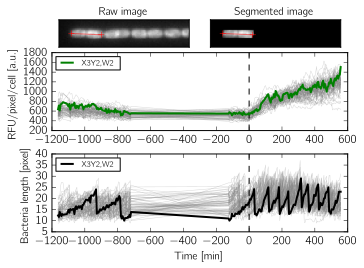
\includegraphics[scale=1]{./Fig/data_acquisition}
\caption{
\textbf{Results of data acquisition.}
We imaged 6 fields (X1Y1, X2Y1, X3Y1, X1Y2, X2Y2, X3Y2) each containing 15 wells (W0 to W14) for $\sim$40 hours.
From this, only 68 wells were available for analysis (the others were either empty, out of frame for some period of time, or plugged).
For all wells, data points are missing in the time interval [-720,-150] because the camera was out of focus.
We stopped the time series analysis at 550 minutes when visually 3/4 of the bacteria were still growing.
The whole population was wiped out in the next few hours for an unknown reason.
The Raw image is the last image analyzed for the highlighted well.
The left bacteria on this image was manually segmented by selecting two pixels at the poles on the fluorescence images (red cross).
A 6-pixel-wide rectangular mask was computed for each image, giving the segmented image on the right.
Fluorescence levels are expressed in Relative Fluorescence Units (RFU) on a 16-bit image (values from 0 to 65335), and were corrected for camera background, but not autofluorescence background (see Material and Methods~\ref{sec:cell_segmentation} and Discussion~\ref{sec:chap3_discussion}).
The RFU/pixel/cell was computed by taking the ratio between the sum of the pixels in the mask, and the total number of pixels in the mask.
The bacteria length is the distance in pixels between the two poles (red line on the raw and segmented images).
The thick lines highlights the time series for the cell visible in the top images.
The dashed black line corresponds to the switch time from acetate to glucose.
}
\label{fig:data_acquisition}
\end{figure}

From this preliminary analysis, we obtained time series for the concentration of fluorescence (RFU/pixel) and the length for 68 bacterial cells (Fig.~\ref{fig:data_acquisition}).
The RFU/pixel appears constant on the acetate phase (before 0) and immediately increases when the medium is switched to glucose.
Bacterial length shows that the division time abruptly decreases after the nutrient upshift, corresponding to a higher growth rate.
Unfortunately, while the steady state on acetate was reached before the upshift, it is obvious that the time series stop before a new steady state on glucose is reached, at least for the fluorescence.
Nevertheless, the time series are not interrupted around the transition.
What do we observe if we estimate the growth rate and $\alpha$ in this region?

\subsection{Data analysis using Kalman smoother}
\label{sec:res_kalman}

As we presented in section~\ref{sec:exp_design}, our goal is to reconstruct the signal $\alpha (\cdot)$ during the transition.
By modeling \textit{E. coli} as a cylinder, the length can be assumed directly proportional to the volume of the cell.
If we assume a negligible background of autofluorescence (see Material and Methods~\ref{sec:cell_segmentation}), the fluorescence concentration in the cell can be assumed proportional to the ribosome concentration.
More precisely, based on the data available, we have the following measurement model at each time-point $t_k$:
\begin{eqnarray}
L(t_k) &= \lambda \cdot V(t_k) + \epsilon_k, \label{eq:mes_L}\\
F(t_k) &= \gamma \cdot r(t_k) + \eta_k, \label{eq:mes_F}
\end{eqnarray}
where $L(t_k)$ (resp. $F(t_k)$) is the length (resp. RFU/pixel) measured at time $t_k$ (visible on Fig.~\ref{fig:data_acquisition}), $V(t_k)$ (resp. $r(t_k)$) is the actual volume (resp. ribosome concentration) at time $t_k$, ($\lambda$,$\gamma$) are unknown proportionality constants, and ($\epsilon_k$,$\eta_k$) are measurement noises.
As we saw in section~\ref{sec:exp_design}, reconstructing $\alpha (\cdot)$ requires information on $\mu (\cdot)$, $r(\cdot)$ and $\dot{r}(\cdot)$.
From Eq.~\ref{eq:mes_F}, we could obtain $r(\cdot)$ and $\dot{r}(\cdot)$ by smoothing interpolation and differentiation.
The same can be said for Eq.~\ref{eq:mes_L} and $\mu (\cdot)$ since it is defined by:
\[
\dot{V}(t) = \mu (t) \cdot V(t).
\]
However, smoothing interpolation is particularly sensible to the boundary conditions.
Since each division in the time series is a boundary, the smoothing interpolation of this kind of data is particularly unstable.
For this reason, single-cell growth rate is usually estimated by fitting an exponential term on the volume between each division (or in particular a linear term on the logarithm of the volume)~[citation Wang et al et Izard et al].
While it is suitable when bacteria are at steady state, it is not applicable in our case where we expect growth-rate variations between divisions.
Other techniques are less sensible to this kind of problem~\cite{zulkower_robust_2015}, and we decided to focus on the use of Kalman smoother~\cite{kailath_linear_2000,jazwinski_stochastic_2007}.

Kalman filtering~\cite{kalman_new_1960} is a bayesian algorithm that uses a series of noisy measurements to predict the state of a dynamical system.
It is well known for its everyday technological applications (guidance, tracking, control, ...) which requires the real-time estimation of hidden variables in a dynamical system based on previous measurements.
Kalman smoothing is an extension of Kalman filtering that uses information about the previous but also the next measurements of the state of the system, and is widely applied to estimate unknown inputs in time series analysis~\cite{kailath_linear_2000,jazwinski_stochastic_2007}.
In that sense, it uses all the available information to estimate the hidden variables of a dynamical system.
For our problem, at each time step $t_k$, our hidden variables are the resource allocation $\alpha (t_k)$ and the growth rate $\mu (t_k)$, and the available information is the N measurements $\left\{ F(t_0), F(t_1), ..., F(t_{N-1}) \right\}$ and $\left\{L(t_0), L(t_1), ..., L(t_{N-1}) \right\}$ that were taken during the whole experiment.

We state the problem as follows.
We have the following dynamical system:
\begin{eqnarray}
\dot{r}(t) &=& \mu (t) \cdot \frac{\alpha(t)}{\beta} - \mu (t) \cdot r(t),\\
\dot{V}(t) &=& \mu (t) \cdot V(t),
\end{eqnarray}
with the following measurement model:
\begin{eqnarray}
L(t_k) &= \lambda \cdot V(t_k) + \epsilon_k,\\
F(t_k) &= \gamma \cdot r(t_k) + \eta_k,
\end{eqnarray}
where each variable has already been defined in Eqs~\ref{eq:dot_r}, \ref{eq:mes_L} and \ref{eq:mes_F}.
While $\beta$ can be obtained from the literature (see chapter~\ref{chap:theory}), $\lambda$ and $\gamma$ are unknown variables that need to be estimated along with $\alpha$ and $\mu$.
Since we are satisfied with a qualitative reconstruction of $\alpha (\cdot)$, we can simplify the system by defining $r_\gamma = \gamma \cdot r$ and $V_\lambda = \lambda \cdot V$.
The dynamical system is thus rewritten:
\begin{eqnarray}
\dot{r_\gamma}(t) &=& \mu (t) \cdot\frac{\gamma \cdot \alpha(t)}{\beta} - \mu (t) \cdot r_\gamma (t),\label{eq:r_prob}\\
\dot{V_\lambda}(t) &=& \mu (t) \cdot V_\lambda (t),\label{eq:V_prob}
\end{eqnarray}
with the new measurement model:
\begin{eqnarray}
F(t_k) &= r_\gamma (t_k) + \eta_k,\label{eq:F_prob}\\
L(t_k) &= V_\lambda(t_k) + \epsilon_k.\label{eq:L_prob}
\end{eqnarray}
The problem becomes the reconstruction of $\gamma \alpha (\cdot) / \beta$ and $\mu (\cdot)$ through measurements $\left\{ F(t_0), F(t_1), ..., F(t_{N-1}) \right\}$ and $\left\{L(t_0), L(t_1), ..., L(t_{N-1}) \right\}$.
Note that this problem is not linear, while Kalman filtering was initially introduced for linear systems~\cite{kalman_new_1960,kailath_linear_2000}.
For this reason, we used a non-linear extension of Kalman smoothing called Unscented Kalman Smoothing~\cite{julier_new_1997,jazwinski_stochastic_2007}.
Details about its exact implementation are available in Material and Methods~\ref{sec:meth_kalman}.
While it is feasible to co-reconstruct the signals $\mu (\cdot)$ and $\gamma \alpha (\cdot) / \beta$ using Kalman smoothing, it is not necessary and could make the reconstruction unstable.
We thus decided to proceed in two steps: first reconstruct $\mu$ from the measurements of $L$, than inject this result in the reconstruction of $\gamma \alpha / \beta$ from the measurements of $F$.

\subsection{Estimation of growth rate and gene expression}

\subsubsection*{Growth rate estimation}

As presented in the previous section, we want to reconstruct the growth rate $\mu$ defined by Eq.~\ref{eq:V_prob}, using measurements of the length $L$ defined by Eq.~\ref{eq:L_prob}.
Note that Kalman smoothing is a procedure that returns the expected mean and covariance of the state of a dynamical system, given some measurements.
Thus, reconstructing $\mu$ requires its explicit integration in the variables of the dynamical system.
In some sense, this tells the system which constraints to apply on the variations of $\mu$, and represents a regularization method.
Here, we used the following Bayesian regularization approach.
In the Kalman smoothing procedure, we model the variations of $\mu$ as the outcome of a stochastic process.
The laws of this process play the role of a prior on the expected regularity of $\mu$ (the more noisy the process, the less constrained the variations of $\mu$).
In particular, we let $\mu$ be the double integral of a Gaussian white noise $w$:
\[
\dot{\mu} = v(t) \;\;\;\; \dot{v} = w(t),
\]
where $v$ is an intermediate variable, and $w(t) \sim \mathcal{N}(0, \theta)$.
The full problem becomes:
\begin{eqnarray}
\dot{V_\lambda}(t) &=& \mu (t) \cdot V_\lambda (t),\nonumber\\
\dot{\mu}(t) &=& v(t),\label{eq:full_mu_prob}\\
\dot{v}(t) &=& w(t),\nonumber
\end{eqnarray}
with the measurement model:
\begin{equation}
L(t_k) = V_\lambda(t_k) + \epsilon_k.
\end{equation}
The advantages of this regularization method are that the reconstructed $\mu$ is guaranteed to be second-order differentiable.
It is also equivalent to other methods like Tikhonov regularization~[citation to take from Val pub], which minimizes least-square differences between predictions and observations along with penalizing the variations of the input.

Our prior is thus entirely contained in the parameters of the Kalman procedure:
\begin{itemize}
\item the mean of the initial state for $V_\lambda$, $\mu$ and $v$,
\item the covariance of the initial state for $V_\lambda$, $\mu$ and $v$,
\item the transition covariance for the derivatives of $V_\lambda$, $\mu$ and $v$,
\item the observation variance for $L$.
\end{itemize}
The means and covariances at the initial state represent the knowledge we have on the initial parameters.
For instance, if we know exactly the value of $V_\lambda$, $\mu$ and $v$, we can fix the means and use very small covariances, but this "certainty" can be adjusted at will.
In our framework, there is no transition covariance for $V_\lambda$ and $\mu$, because there are not the result of a stochastic process.
However, the transition variance $\theta^2$ of the derivative of $v$ is crucial: it represents the intensity of the white noise $w$ that serves as prior for the regularization of $\mu$.
The smaller its value, the more the variations of $v$ are penalized, hence the smoother the reconstructed $\mu$.
Finally, the observation variance for $L$ is the expected measurement noise.
All these parameters represent the prior that we use to reconstruct the growth rate $\mu$.
As we will see below, we widely use these properties to overcome the difficulties raised by the discontinuities introduced by cell divisions.

Since we track bacteria for a long time, the observation of their length $L$ is inherently discontinuous, due to symmetrical divisions of the \textit{E. coli} cells (Fig.~\ref{fig:data_acquisition}).
Thus, the problem cannot be solved for the whole time series at once, but has to be divided into smaller continuous regions between two divisions.
We simply localize the divisions by looking at the time points at which the empirical derivative of the length is below an arbitrary threshold, and slice the curve into the appropriate number of continuous time series.
From here, the most straightforward method would be to treat each portion independently.
However, we loose an important information by doing so: neighbor portions of the curve are likely to have similar growth rate.
This comes from the fact that we can expect a daughter cell to start growing with a growth rate similar to its mother cell.
In other word, while not necessary continuous, the growth rate at the boundaries of a time region can be expected to depend strongly on the growth rate of neighbor regions.
This can be easily taken into account in the Kalman smoothing procedure by exploiting the priors about the initial mean and covariance of the system variables.
We simply let the initial state mean of the growth rate be the last estimated value in the mother cell, while defining a reasonable variance around this value to allow flexibility.
When no data about the mother cell is available (at the beginning of the experiment), we simply let the algorithm choose freely the initial growth rate by defining a large variance around the expected growth rate on acetate.
The results of this procedure, along with the exact parameters used for the Kalman smoothing, are reported in Fig.~\ref{fig:growth_rate_estimation} and Material and Methods~\ref{sec:meth_kalman}.

\begin{figure}[p]
\centering
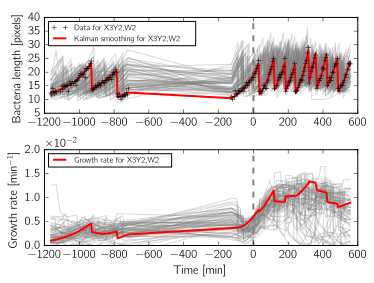
\includegraphics[scale=1]{./Fig/growth_rate_estimation}
\caption{
\textbf{Growth rate estimation based on the bacterial length using Kalman smoothing.}
Grey lines represent estimation of states of the system by the unscented Kalman smoothing procedure for the 68 cells.
The reconstruction for the bacterial length and the growth rate are presented in the top and bottom graphs, respectively.
For readability, the solid red lines highlight the result for a particular cell, while black crosses in the top graph are the data points for this cell.
The dashed grey lines represent the switch time from acetate to glucose.
As prior for the algorithm, we used an observation variance of 9 pixels\textsuperscript{2} for the length $L$.
The transition variance $\theta^2$ (\textit{a.k.a.} the smoothing factor for $\mu$) is fixed at $10^{-8}$~min\textsuperscript{-6} during the whole time series.
Inheritance between mother and daughter cells is taken into account by systematically choosing an initial mean equal to the last estimated value for $\mu$, and to half the last estimated value for $V_\gamma$ (modeling the symmetrical division).
At the beginning of the experiment, were no mother cell is available, these values were fixed at 15~pixels for $V_\gamma$ and 0.004~min\textsuperscript{-1} for $\mu$.
The variances associated with these means are 16~pixels\textsuperscript{2} and $10^{-4}$~min\textsuperscript{-2}, respectively for $V_\gamma$ and $\mu$.
$v$ initial mean is always taken null, with an initial variance of $10^{-8}$~min\textsuperscript{-6}.
All the cross-covariances are set to 0 because the system variables are independent by construction.
The parameters cited above were chosen through trials and errors, and are as a consequence largely optimizable.
Possible improvements are discussed in section~\ref{sec:chap3_discussion}.
}
\label{fig:growth_rate_estimation}
\end{figure}

On the mean, the results presented in~Fig.~\ref{fig:growth_rate_estimation} show a roughly constant growth rate on acetate, followed by a quick increase around the upshift.
Contrary to what was visible on the fluorescence, a steady state for the growth rate seems to have been reached before the end of the experiment.
When taken individually, the results are more fuzzy.
A significant part of the cells stops growing before the end of the experiment.
This was expected since all the cells die from an unknown cause at the end of the time series, and the interval of analysis was visually chosen so that roughly 3/4 of the cells are still growing.
Interestingly, 1/6 of the cells exhibit growth rate oscillations, with a hour-long pause around 200 minutes after the upshift, then a growth rate recovery until the end of the time series (see Supporting Information XX).
For now, we decided to classify the cells in three categories: the dying cells (N=12) for which the growth rate drop to zero after the upshift; the pausing cells (N=11) for which the growth rate drop to zero after the upshift then recover, and finally the normal cells (N=45) which do not exhibit any of the above behaviors.
More information about each category is available in Supporting Information XX.
In what follows, we focus on the 45 normal cells (Fig.~\ref{fig:growth_rate_estimation_median}), which present a globally coherent behavior until the end of the interval of analysis.

\begin{figure}[tb]
\centering
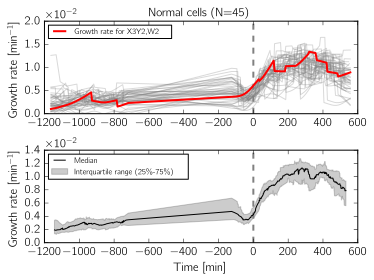
\includegraphics[scale=1]{./Fig/growth_rate_estimation_median}
\caption{
\textbf{Growth rate estimation for the normal cells only.}
The top graph is the same as the bottom graph of Fig.~\ref{fig:growth_rate_estimation}, except we removed the dying and pausing cells.
The bottom graph gives the 25\% (lowest gray line), 50\% (solid black line) and 75\% (highest gray line) quartiles, computed at each time step.
The gray area represents the interquartile range.
}
\label{fig:growth_rate_estimation_median}
\end{figure}

\subsubsection*{Estimation of gene activity}

We use a similar Bayesian regularization approach than for the growth rate estimation.
We note $u(t) = \gamma \alpha (t) / \beta$ the input that we want to reconstruct.
The full problem for the estimation of $u$ is:
\begin{eqnarray}
\dot{r_\gamma}(t) &=& \hat{\mu} (t) \cdot u (t) - \hat{\mu} (t) \cdot r_\gamma (t), \nonumber\\
\dot{u}(t) &=& v(t),\label{eq:full_u_prob}\\
\dot{v}(t) &=& w(t),\nonumber
\end{eqnarray}
with the measurement model
\begin{equation*}
F(t_k) = r_\gamma (t_k) + \eta_k,\\
\end{equation*}
where $\hat{\mu}$ is the estimation of $\mu$ from the previous section.
Contrary to the growth rate problem, this system is linear.
Furthermore, we do not have to deal with discontinuities of the measurement since $F$ is continuous from the mother to the daughter cells (Fig.~\ref{fig:data_acquisition}).

To be comparable with what we predicted in chapter~\ref{chap:theory}, we expect $u(\cdot)$ to exhibit bang-bang variations after the upshift.
By definition, it is a very stiff signal that could be complicated to reconstruct depending on the parameters of the regularization method.
In order to parametrize the Kalman smoothing algorithm, we generated synthetic data by simulating the model of chapter~\ref{chap:theory}.
This was not possible for the growth rate problem since cell division is absent from the model.
After estimating the noise on the RFU/pixel measurements (see Supporting Information XX), we simulated an upshift from acetate to glucose (the parameters were chosen based on the resulting growth rate), and used a value for $\gamma$ that generated a fluorescence concentration in the range of the observations.
We then tried to estimate $\gamma \alpha / \beta$ based these synthetic data, choosing the prior parameters through trials and errors.
There are probably not optimal, and we discuss possible improvements in section~\ref{sec:chap3_discussion}.
The results along with the prior parameters are presented in Fig.~\ref{fig:synthetic_upshift}.
Like any smooth methods, the algorithm has trouble reconstructing stiff variations of the system variables.
The oscillatory nature of gene expression is however fully captured, which indicate that the algorithm should be able to conclude on the existence of the \textit{on-off} strategy.
Some methods that could improve this result are also discussed in section~\ref{sec:chap3_discussion}.
In what follows, we use the same prior parameters on the "normal cell" subset of the real data, in order to see if we can get the same oscillatory pattern.

\begin{figure}[p]
\centering
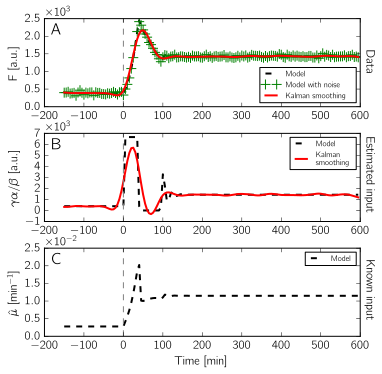
\includegraphics[scale=0.8]{./Fig/synthetic_upshift}
\caption{
\textbf{Performance of the unscented Kalman smoother on synthetic data simulating an upshift.}
\textit{(A)}~Synthetic data simulating an upshift with and without white noise, along the result of the Kalman smoothing procedure.
The synthetic data were generated by simulating the model presented in Eqs~\ref{eq:pdef}-\ref{eq:rdef} with the on-off regulatory strategy (Eq.~\ref{eq:stratswitch} and Fig.~\ref{fig:onoffresults}).
Parameters for the simulation are $e_{M,\texttt{Ace}} = 0.18$~h\textsuperscript{-1}, $e_{M,\texttt{Glu}} = 0.9$~h\textsuperscript{-1}, $k_R = 3.6$~h\textsuperscript{-1}, $\beta = 0.003$~L.g\textsuperscript{-1}, $K_R = 1$~g.L\textsuperscript{-1}.
The simulated $r(t)$ was multiplied by a factor $\gamma = 0.02$~L.g\textsuperscript{-1}.RFU\textsuperscript{-1} in order to get a synthetic $F$ in the same range of the observations (dashed black curve).
Additive noise level was estimated from the real data and injected in $F$ (see Supporting Information XX).
Here again, the parameters were chosen through trials and errors, and are reported in the Material and Methods~\ref{sec:meth_kalman}.
They are largely optimizable, and possible improvements are discussed in section~\ref{sec:chap3_discussion}.
\textit{(B)}~Estimation of $\gamma \alpha / \beta$ based on the data in (A).
As described in chapter~\ref{chap:theory}, $\alpha (t)$ performs a bang-bang-singular response during the upshift (dashed black line).
While the Kalman smoothing is not able to capture the stiff variations of $\gamma \alpha / \beta$, it fairly reproduces the oscillatory nature of the gene expression (red solid line).
\textit{(C)}~The growth rate during the upshift.
This information is used as an input in the procedure, since it is supposed to have been independently estimated from the measurements $\left\{L(t_0), L(t_1), ..., L(t_{N-1}) \right\}$.
}
\label{fig:synthetic_upshift}
\end{figure}

Results of the reconstruction of $u = \gamma \alpha / \beta$ are presented in Fig.~\ref{fig:gene_activity}.
Large oscillations are indeed visible on the reconstruction.
These oscillations were already visible on the RFU/pixel data (Fig.~\ref{fig:gene_activity}A).
The region between -150 and 0 min appears to be the most stable, as we could expect for a growth steady state.
On the contrary, the reconstructed $\gamma \alpha / \beta$ seems particularly unstable at the beginning and the end of the experiment.
Overall, the oscillations observed must be taken with extreme caution.
The problem of reconstructing an on-off signal is more challenging than we initially thought, for the simple reason that the signal we expect to reconstruct is exactly the kind of artifacts a poorly calibrated regularization method would generate.
Data about the pre-upshift and post-upshift steady state are more crucial than expected, and the experimental problem we described earlier truly impedes our capacity to conclude on the regulatory strategy.
We extensively discuss this in section~\ref{sec:chap3_discussion}, and give numerous indications about the future improvements that will be implement.
Finally, Fig.~\ref{fig:gene_activity_median} gives an idea of the distribution of the estimations at each time step.
While most oscillations cancels out when we consider global statistics about the population, the first oscillation just after the upshift is conserved in each of the 25\%, 50\% and 75\% quartiles (Fig.~\ref{fig:gene_activity_median}B).
This is rather encouraging and prompts for future investigations.

\begin{figure}[p]
\centering
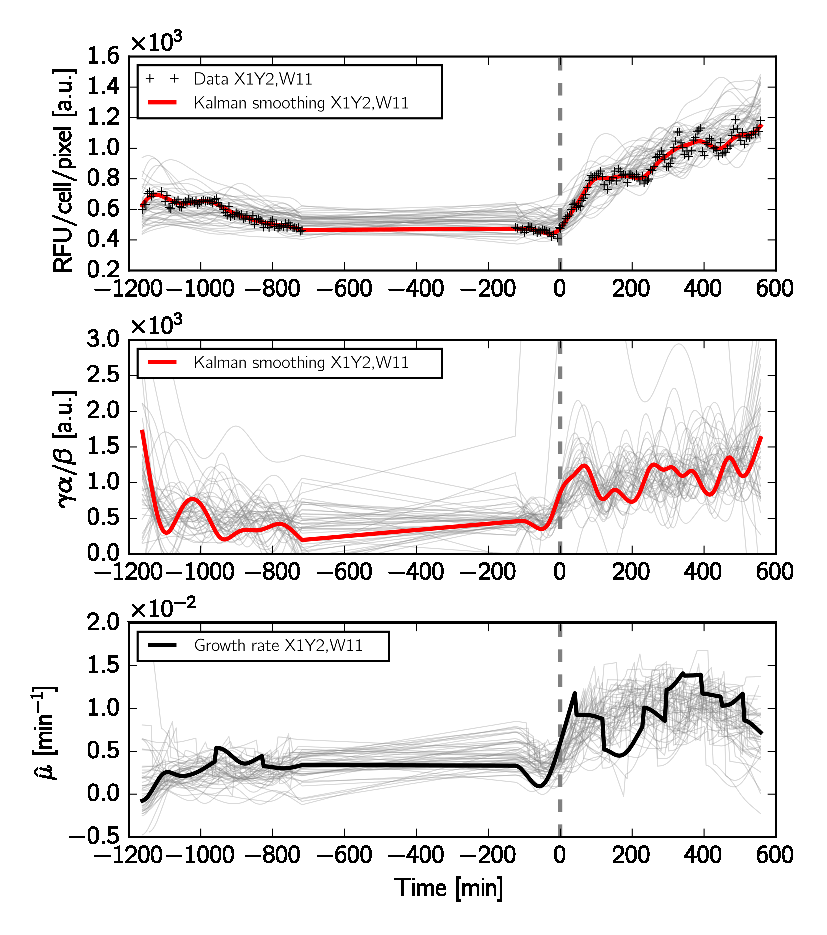
\includegraphics[scale=1]{./Fig/gene_activity}
\caption{
\textbf{Gene activity estimation based on the RFU/pixel measurements using Kalman smoothing.}
\textit{(A-B)} Grey lines represent estimation of state of the system by the unscented Kalman smoothing procedure for the 45 normal cells.
For readability, the solid red lines highlight the result for a particular cell, while black crosses in the top graph are the data points for this cell.
The dashed grey line represents the switch time from acetate to glucose.
The reconstruction for the RFU/pixel measurements and the gene activity $\gamma \alpha / \beta$ are presented in the (A) and (B), respectively.
The prior parameters used for the algorithm are exactly the same than in Fig.~\ref{fig:synthetic_upshift} and are reported in Material and Methods~\ref{sec:meth_kalman}.
}
\label{fig:gene_activity}
\end{figure}

\begin{figure}[p]
\centering
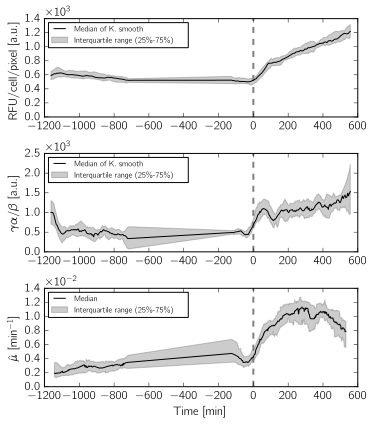
\includegraphics[scale=1]{./Fig/gene_activity_median}
\caption{
\textbf{Distribution of the estimation results presented in Fig.~\ref{fig:gene_activity}.}
Interestingly, while most oscillations in $\gamma \alpha / \beta$ are canceled out at the population level, the first one after the upshift is conserved.
Each graph gives the 25\% (lowest gray line), 50\% (solid black line) and 75\% (highest gray line) quartiles, computed at each time step for the signals reconstructed in Fig.~\ref{fig:gene_activity}.
The gray area represents the interquartile range.
}
\label{fig:gene_activity_median}
\end{figure}

\section{Discussion}
\label{sec:chap3_discussion}

As we showed in chapter~\ref{chap:theory}, adopting a dynamical perspective might prove useful to unveil and understand the regulatory strategies employed by microorganisms.
The criteria of biomass optimization has proved useful to uncover and explain the steady-state empirical growth laws.
Interestingly, when the same criteria are applied in growth transitions, they suggest that microorganisms should converge toward a bang-bang control of gene expression.
For the control of ribosome synthesis, this would result into implementing an \textit{on-off} regulatory system, either only producing ribosomes, or not producing them at all, during the adaptation to the new growth medium.
The widespread ppGpp system, known for its role in the control of ribosome synthesis, is theoretically able to implement such a regulatory system.
But we lack experimental data to show that it does so, mostly because of the difficulties raised by working in growth transitions.
Can we measure the ribosomal synthesis rate at the single-cell level during well-controlled growth transitions?
Would it exhibit the \textit{on-off} strategy that was shown to be close to optimal in chapter~\ref{chap:theory}?

In this chapter, the above questions have been addressed by developing an experimental framework which allows the relative ribosome concentration to be estimated at the single-cell level in real time on \textit{E. coli}.
Our main contribution consists into bringing together several experimental breakthroughs of the recent years.
On one hand, inspired by the work of Bakshi \textit{et al}~\cite{bakshi_superresolution_2012}, we reconstructed a \textit{E. coli} strain displaying fluorescent, but still fully effective, ribosomes.
In their paper, Bakshi \textit{et al} essentially used it to localize ribosomes in the cytoplasm through superresolution microscopy.
While improving their design (see Material and Methods~\ref{sec:methods_strain}), we used it for the purpose of quantifying the ribosomal abundance.
On the other hand, we used the mother machine~\cite{wang_robust_2010} developed by Wang \textit{et al} to observe this strain growing in continuous culture through real-time microscopy.
This microfluidic device was originally developed to study long-term steady-state growth of \textit{E. coli}.
Here, we used it to observe growth transitions in a well controlled framework, \textit{i.e.} from one steady-state growth to another steady-state growth.
By changing the medium that was injected into the device, we were able to observe \textit{E. coli} transitioning from growth on acetate to growth on glucose.
Overall, through the combination of fluorescent labeling of a core component of the gene expression machinery and the use of a microfluidic device, we opened the way to the experimental study of growth laws in a dynamical context.

We applied this experimental set-up to the reconstruction of the resources allocation strategy employed by \textit{E. coli} during an environmental upshift.
Obviously, the goal was to eventually observe the oscillations predicted in chapter~\ref{chap:theory}.
We applied a signal processing algorithm known as Kalman smoothing and showed how it can be implemented to reconstruct the inner state of a cell from microscopy data.
Similar to hidden markov chains, Kalman filtering and smoothing are powerful techniques allowing the reconstruction of hidden signals from noisy measurements, and have already numerous everyday applications, though not so much in biology.
We showed in this chapter that the Bayesian logic behind Kalman smoothing can be exploited to inject in the growth rate reconstruction, a probabilistic prior that define the relation between the mother and its daughter cells.
We also applied it for the reconstruction of $\alpha$, the abstract resource allocation parameter defined in chapter~\ref{chap:theory}.
Our work on synthetic data showed that despite being challenged by the high stiffness of the signal, the algorithm was able to fully recover the oscillatory pattern that we expect to occur \textit{in vivo}.
Unfortunately, its application on our dataset was not so successful: while oscillations can be reproduced, the signal is not strong enough to distinguish whether the oscillations are real or chimerical.
We propose below several improvements that will certainly be addressed in future work.

Several experimental problems dramatically impeded the analysis of the data.
Sufficiently long steady-state measurements before and after the transition of interest are needed to provide a strong estimation of the intensity and the nature of the experimental noise.
They are also critical to calibrate the parameters of the regularization method used in the signal reconstruction.
Despite what was initially planned, we did not get long enough steady-state measurements far from the transition.
Several causes are to blame.
First, the random stall of the motorization along the Z-axis of the microscope, which do not allow overnight measurements and occurred during the slow growth on acetate in the presented experiment.
Secondly, the massive death of bacteria starting after the transition on glucose.
Future work will focus on solving these issues.

The death of bacteria is particularly worrying.
During the construction of this strain, most people in the lab experienced contamination by an aggressive bacteriophage.
Unfortunately, the strain used in this study was not spared, and our frozen stocks were later tested positive for phage-induced lysis.
Interestingly, the lysis seems to depend strongly on the environmental conditions.
To our disarray, the massive death observed in this experiment suggests that a strong environmental upshift could trigger the lytic cycle of the phage.
While impeding any possible long-term measurement, the death of the bacteria is not our only worry.
Phages are machines that are extremely well optimized to divert cell resources to their own end, especially the activity of the gene expression machinery.
That could dramatically perturb the cell regulation of resource allocation, and so the conclusions of this study.
For this reason, future work will start by the reconstruction of a clean phage-free strain from scratch.

The data analysis technique used is also largely optimizable.
The results reported here are largely preliminary.
We segmented the images using the most powerful and ubiquitous segmentation algorithm available: the human brain.
In other word, we manually selected the pixels representing the poles of a single bacteria per well on the fluorescence images, and used this information to arbitrarily define a mask around the cell of interest.
This is far from satisfying.
Unfortunately, it seems that the first rule of image analysis is that every application is more or less unique.
Every algorithm has to make assumptions about the object it is trying to recognize.
For bacteria imaging, it could be the curvature at the poles, the size of the pixels, the homogeneity of the background, the homogeneity of the inner fluorescence...
While some parameters can be tweaked, some assumptions are always hard-coded in the algorithm and reflect the philosophy used to address the identification problem.
Since this preliminary analysis was made, we started a collaboration with the authors of FluoBacTracker~[citation, ask Hugues if a publication exist] that focuses on adapting their software to our set-up in a near future.
It should provide a robust, automatic way to identify and track the cells, enhancing reproducibility of the analysis.

The signal reconstruction algorithm that was later applied to these data is also largely optimizable.
Like we described in the previous section, the algorithm is an instance of Bayesian reconstruction.
Several parameters describing the expected input define a probabilistic prior.
Preliminary, we chose these parameters through trials and errors, or by calibrating the system on synthetic data when it was possible.
A better technique would be to choose these parameters by \textit{generalized cross-validation} (GCV)~\cite{golub_generalized_1979}, a procedure that maximizes the predictive power of the reconstructed signal.
More generally, parameters could be optimized on a subset of the cells, then tested against the remaining subset.
It would ensure that the algorithm does not overfit the behavior of a few cells.
While the initial conditions did not seem to play a huge role in the final shape of the signal, the choice of the smoothing factor $\theta^2$ appeared to be critical, and would strongly benefit from such an implementation.

We also did not fully exploited the power of Kalman smoothing.
Smoothing methods have trouble estimating abrupt transitions, and our implementation has the same issue.
As we can see in Fig.~\ref{fig:synthetic_upshift}, the reconstructed signal for $\gamma \alpha / \beta$ increases before the shift actually happen.
This artifact also appears for the real data (Fig.~\ref{fig:gene_activity_median}), were the signal start to change dozens of minutes before the shift.
We know exactly when bacteria start to be in contact with the new medium, but this information is never used as prior for the reconstruction.
Using this information is however possible with Kalman smoothing.
By implementing time-varying parameters for the regularization method, we can strongly penalize the variations of the reconstructed signal at steady state (when nothing is expected to happen) and release the constraints as soon as the medium is changed (when we expect most of the stuff to happen).
Such a method has already been successfully applied to correctly estimate changes in growth rate during sugar exhaustion~[citation in preparation Eugenio].

We are convinced the improvements cited above would allow to robustly conclude on the existence of the on-off strategy, and are not excessively hard to implement.
Other more challenging developments are planed and would probably benefit to the framework as a whole.
For instance, we did not discuss the autofluorescence of the bacteria in this chapter.
It was assumed negligible, mostly because its proper estimation in a dynamical, single-cell context is complicated (see Material and Methods~\ref{sec:cell_segmentation}).
Nevertheless, a simple trick could solve the issue: merging wild-type and fluorescent bacteria when inseminating the device.
The goal would be to have a significant part of the channels occupied by wild-type cells, while still being able to observe in parallel the strain of interest.
That way, we could have an exact estimation of the level of autofluorescence of the cells, and robustly correct it for the channels of interest.
Note that this would reduce the amount of exploitable channels, hence would probably require several adjustments. 

Something is also displeasing in the current implement of the Kalman smoothing method.
As described in the main text, the Kalman smoothing procedure not only use previous measuments to estimate the state of the system, but also the next available measurements.
This is a feature we totally lose in the estimation of the growth rate, because the discontinuities introduced by the cell divisions impede a global analysis of the time series.
We partially solved the issue by using information about the mother cell at the beginning of the growth rate reconstruction of the daughter cells, but we did not find a way to implement it backward.
There is probably a better way to deal with cell division in the analysis of microscopy data, and we are actively working on the matter.

\section{Material and Methods}

\subsection{Bacterial strain construction}
\label{sec:methods_strain}

To achieve dynamical quantification of ribosome abundance, we designed and constructed a strain containing a translational fusion of \textit{gfpmut2}~\cite{zaslaver_comprehensive_2006} to the C-terminus of \textit{rpsB} (the gene coding the ribosome subunit S2).
This design was inspired by the work of Bakshi \textit{et al}, who used a similar construction to assess the quantitative spatial distribution of ribosomes in living \textit{E.~coli}~\cite{bakshi_superresolution_2012}.

The transcription factor \textit{tsf} is under the control of the same promoter than \textit{rpsB}, and is located after the C-terminus.
In order to ensure that \textit{tsf} expression was not affected by our translation fusion on \textit{rpsB}, we used a double-selection procedure to get rid of every resistance gene that the construction might introduce.
This is something that was not done in the original construction from Bakshi \textit{et al}~\cite{bakshi_superresolution_2012}

A DNA fragment containing a double selection cassette was amplified with two long primers annealing respectively to the region just after the STOP codon at the C-terminus of \textit{rpsB}, and to the beginning of \textit{gfpmut2}.
The double-selection cassette contained a resistance gene to Kanamycin (positive selection) and a gene coding for the CcdB toxin under the control of the P\textsubscript{BAD} promoter (negative selection in presence of Arabinose).
This cassette is referred below as \textit{kan-P\textsubscript{BAD}-ccdB}.

Another DNA fragment containing \textit{gfpmut2}~\cite{zaslaver_comprehensive_2006} without ATG was amplified with long primers annealing respectively to the C-terminus of \ref{chap:theory}rpsB (just before the STOP codon), and the end of the \textit{kan-P\textsubscript{BAD}-ccdB} cassette.
The first primer also contained a 18-bp (base pair) linker that was chosen according to the method section of~\cite{bakshi_superresolution_2012}.

Both fragments (the \textit{gfpmut2} reporter and the \textit{kan-P\textsubscript{BAD}-ccdB} cassette) were assembled using Gibson assembly~\cite{gibson_enzymatic_2009}.
Both PCR products were quantified using NanoDrop and mixed in equimolar proportions with a commercial Gibson Assembly Master mix.
A final product of 2683 bp was obtained:
\begin{itemize}
\item *(50 bp) the C-terminus of \textit{rpsB} without the STOP codon 
\item (18 bp) a linker (see Supporting Information)
\item (714 bp) the \textit{gfpmut2} sequence without the initial ATG
\item (1851 bp) the \textit{kan-P\textsubscript{BAD}-ccdB} cassette
\item *(50 bp) the region directly after \textit{rpsB} in \textit{E.~coli}
\end{itemize}
Regions labeled with * are expected to anneal with the \textit{E.~coli} chromosome.
The complete sequence of this fragment, as well as all the primers used are available in the Supporting Information of this chapter.

This fragment was electroporated in a BW25113 background strain containing the pSIM5 plasmid with chloramphenicol resistance (lambda-red recombinaison).
A kanamycin-resistant colony was selected and verified to exhibit green fluorescence in a Tecan microplate reader.
A new 100-bp fragment containing 50 bp of the end of \textit{gfpmut2} and 50 bp of the region just after \textit{rpsB} was electroporated into this strain (sequence available in Supporting Information) to get rid of the \textit{kan-P\textsubscript{BAD}-ccdB} cassette.
An arabinose-resistant colony was selected and verified to be kanamycin-sensitive and to still exhibit green fluorescence.
Finally, the strain was grown overnight at 42$^\circ$C to get rid of the pSIM5 plasmid and a chloramphenicol-sensitive colony was selected.
The region after \textit{rpsB} was verified by sequencing (full sequence available in Supporting Information).

In parallel, the same protocol was used to construct \textit{mCherry} and \textit{cfp} variants of the same strain.
However, only the \textit{gfpmut2} and \textit{mCherry} versions were successfully obtained for reasons that were not investigated.
The full sequence of the final \textit{rpsB-mCherry} strain is available in Supporting Information.

The \textit{rpsB-gfpmut2} and \textit{rpsB-mCherry} strains were characterized on different media using a Tecan microplate reader.
They were showed to exhibit a wild-type growth rate and sufficient fluorescence level to allow quantification.
However, the \textit{rpsB-mCherry} strain exhibited strange fluorescence dynamics, especially during growth transitions, which made it unsuitable for our study.
Our effort were then concentrated on the \textit{rpsB-gfp} strain.
Data as well as information on the matter are available in Supporting Information.

\subsection{Growth conditions}
\label{sec:growth_condition}

Sterilization was performed by autoclaving for instruments and filtration for solutions (0.2 $\mu$m).
During cloning, bacteria were grown in 20-mL flasks filled with LB or spread on Petri dish with LA.
In all the experiments, we used M9 minimal medium~[citation to find] supplemented with trace elements, thiamine and a carbon source.
The full recipe is reproduced below.
Numbers in squared brackets are characteristics of the stock solution.
All stock solutions were stored at room temperature, except for FeSO$_4$~[30 g.L\textsuperscript{-1}] and Thiamine~[10 g.L\textsuperscript{-1}] that were stored respectively at -20$^\circ$C and 4$^\circ$C.
\begin{center}
\begin{tabular}{|l r|}
  \hline
  \multicolumn{2}{|c|}{\textbf{M9 medium (100 mL)}}\\
  \hline
  CaCl2 [1 mol.L\textsuperscript{-1}] & 10 $\mu$l\\
  MgSO$_4$ [1 mol.L\textsuperscript{-1}] & 200 $\mu$l\\
   5x Salts & 20 mL \\
  Traces elements & 90 $\mu$l \\
  FeSO$_4$ [30 g.L\textsuperscript{-1}] & 10 $\mu$l \\
  Thiamine [10 g.L\textsuperscript{-1}] & 50 $\mu$l \\
  Carbon source & at will \\
  H$_2$0 [18.2 M$\Omega$.cm] & to 100 mL \\
  \hline
\end{tabular}
\begin{tabular}{|l r|}
  \hline
  \multicolumn{2}{|c|}{\textbf{Traces elements (0.9 mL)}}\\
  \hline
  H$_2$0 [18.2 M$\Omega$.cm] & 200$\mu$l\\
  Na$_2$EDTA 2H$_2$O [150 g.L\textsuperscript{-1}] & 100$\mu$l\\
  ZnSO$_4$ 7H$_2$O [45 g.L\textsuperscript{-1}] & 100$\mu$l\\
  CoCl$_2$ 6H$_2$O [3 g.L\textsuperscript{-1}] & 100$\mu$l\\
  MnCl$_2$ 4H$_2$O [10 g.L\textsuperscript{-1}] & 100$\mu$l\\
  H$_3$BO$_3$ [10 g.L\textsuperscript{-1}] & 100$\mu$l\\
  Na$_2$MoO$_4$ 2H$_2$O [4 g.L\textsuperscript{-1}] & 100$\mu$l\\
  CuSO$_4$ 5H$_2$O [3 g.L\textsuperscript{-1}] & 100$\mu$l\\
  \hline
\end{tabular}
\begin{tabular}{|l r|}
    \hline
  \multicolumn{2}{|c|}{\textbf{5x Salts (100 mL)}}\\
  \hline
  Na$_2$HPO$_4$2H$_2$0 & 4.25 g \\
  KH$_2$HPO$_4$ & 1.5 mg \\
  NaCl & 0.25 g\\
  NH$_4$Cl& 0.5 g\\
  H$_2$0 [18.2 M$\Omega$.cm] & to 100 mL \\
  \hline
\end{tabular}
\end{center}

A large quantity of M9 was prepared several days before the experiment, and stored at 4$^\circ$C.
It contained all the necessary components except FeSO$_4$, thiamine, and carbon sources that were added the day the pre-culture were launched.
Except stated otherwise, the growth temperature was 37$^\circ$C.
M9 Acetate contains 0.2\% Acetate (in mass of C$_2$H$_3$O$_2$ per mass of solution), and M9 Glucose contains 0.2\% Glucose (in mass of D-(+)-Glucose per mass of solution).

At J-4, the glycerol stock containing the \textit{rpsB-gfp} strain was spread out on a Petri dish of LA, and incubated at 37$^\circ$C.
At J-3, an isolated colony was inseminated in 20 mL of M9 Acetate, and incubated in a cotton-plugged sterile flask (Fig.~\ref{fig:experiment_schema}).
Time of insemination was calculated to obtain a 0.3-0.4 cm\textsuperscript{-1} OD when starting the experiment, which correspond to a mid-exponential phase.

At J+0, the preculture was concentrated by centrifugation and back suspended into 5 mL of M9 Acetate supplemented with 50 mg.mL\textsuperscript{-1} BSA (passivation	buffer) for injection into the microfluidic device.
Channels were populated by diffusion until most of them were filled with cells ($\sim$1 hour).
Data acquisition started after a constant medium flow was successfully obtained ($\sim$1 hour, depending on the quality of the device).

\subsection{Microfluidic device}
\label{sec:microflu}

We used the mothermachine~\cite{wang_robust_2010}.
It consists of a series of growth wells (or channels), oriented at a 90$^\circ$ angle to a large central channel through which growth medium is passed at a constant flow.
The wideness of the wells is selected as to constrain the growth direction of the bacteria.
This design ensures that at least one cell per well (the deepest one) is preserved during the whole experiment, while the others incrementally escape into the central channel as divisions occur.
For the fabrication of the devices, we thoroughly followed the step described in the supporting information of~\cite{wang_robust_2010}.
We maintained a stock of chemically treated devices at room temperature (day 2 in workflow summary~\cite{wang_robust_2010}).
The day of the experiment, a single device was plasma cleaned, bond to a glass coverslip, and injected with bacteria (see section above).

The device was connected using 0.023" inner diameter polyethylene tubes to a waste and a sterile bottle containing 200 mL of growth medium, which was enough for several days of acquisition.
A microfluidic pump (Elvesys) containing an output flow sensor module was plugged to the medium bottle, and was applied a pressure up to 2 bars.
The output flow was set to 50 $\mu$L.min$^{-1}$.

For the imaging, the device was placed on a motorized inverted microscope (Zeiss Axiovert 200M) with a phase contrast objective lens (Zeiss PlanNeofluar, Ph3 100x/1.3), placed in a thermostated box at 37$^\circ$C.
In this setup, fluorescence illumination is provided by a mercury lamp (Osram, 1xHBO 103X/2) and visualization is performed with narrow-bandpass excitation and emission filters (Chroma, \#49002 ET-GFP and Chroma, \#49005 TR/DsRED ET).
The exposure time to the light source is externally controlled by mechanical shutters (Uniblitz-VS35).
Images are acquired with a 16-bit gray level CCDcamera cooled to -80$^\circ$C (Roper Scientific, Princeton Instruments PHOTOMAX 512) controlled by a custom-made software using Visual Basic and the Type libraries of the Winview software (Princeton Instruments).
Every 5 minutes, autofocus was numerically performed by maximizing the contrast of a region of interest, and a serie of acquisitions was made.
A total of 6 fields, each containing 15 wells was observed during the whole experiment.

\subsection{Cell segmentation}
\label{sec:cell_segmentation}

Raw data are in the form of 512x512-pixel 16-bit SPE images (proprietary format produced by the Princeton Instruments camera).
They were converted in 16-bit Tif images using the \textit{SPE} plugin of ImageJ~\cite{goto_open_2005}.
The rest of the analysis was performed using Python 3.5.2.
In particular, we used OpenCV~3.1.0-dev, Scikit-Image~0.12.3, Numpy~1.11.2 to manipulate the images.

The offset between consecutive images of a given field was evaluated using cross-correlation in the Fourier space~\cite{guizar-sicairos_efficient_2008} (see Scikit-Image documentation at \cite{skimage_cross-correlation}).
All the images for a field were then aligned on the first acquisition by simple affine translation.

The wells were isolated in individual images through a combination of manual pixel selection and automatic segmentation.
In particular, we selected the entrance of the two wells at the border of the image, and used this information along with the regularity of the microfluidic device to compute a mask that allowed to crop each well in its own image of size 100x21 pixels.
These sub-images were labeled $\left\{W0, W1, ..., W14\right\}$ depending on the position of the well on the original image, from left to right.

In this study, we performed a preliminary analysis on each well that focused on the deepest cell.
For each image, we manually selected two pixels representing the position of the poles of the cell of interest.
The distance between the two selected pixels was directly used as the bacteria length $L$ in pixels.
They were also used to compute a rectangular 6-pixel-wide mask around the cell (see Fig.~\ref{fig:data_acquisition}).
We then computed the RFU/pixel in this cell mask by summing each pixel and dividing by the mask size.

The camera noise and background was evaluated by taking a picture with a closed shutter at the end of the experiment.
Pixels in this picture were found to be Gaussian distributed with a mean of 1101.0 and a standard deviation of 10.788.
Correction for camera background was thus applied by removing 1101 to the computed RFU/pixel.

The background for autofluorescence of the bacteria and the medium was supposed negligible and was thus not corrected.
Indeed, the same device was used to image bacteria in stationary phase that do not produce any fluorescent protein.
They were entirely indistinguishable from the camera noise.
Not that this does not ensure that the autofluorescence is also negligible when the bacteria are actively growing.
Furthermore, its value could change with the medium of interest, and even be different at steady state and during growth transitions, which does not allow to estimate it independently.
In the section~\ref{sec:chap3_discussion}, we discuss possible improvements of the experimental set-up that would allow to dynamically co-estimate the autofluorescence with the ribosome abundance in a single experiment.

\subsection{Kalman smoothing}
\label{sec:meth_kalman}

The data about the length and the RFU/pixel of each bacteria were analyzed using Python~3.5.2.
In particular, we manipulated the data using Pandas~0.19.1, pykalman~0.9.5 and the curves submodule of wellfare~0.1.1.

Historical details about the Kalman smoothing procedure are reported in section~\ref{sec:res_kalman} of the main text.
We used the Additive Unscented Kalman Filter implementation of the pykalman python module.
This class is reported to be more stable and computationally efficient with non-linear problems featuring additive noises.

As described in section~\ref{sec:res_kalman}, the reconstruction of the growth rate was done on continuous portions of the length, \textit{i.e.} between two division events.
The full problem, as reported in Eq.~\ref{eq:full_mu_prob}, is reproduced below for clarity is:
\begin{eqnarray*}
\dot{V_\lambda}(t) &=& \mu (t) \cdot V_\lambda (t),\nonumber\\
\dot{\mu}(t) &=& v(t),\\
\dot{v}(t) &=& w(t),\nonumber
\end{eqnarray*}
with the measurement model:
\begin{equation*}
L(t_k) = V_\lambda(t_k) + \epsilon_k.
\end{equation*}
The parameters used as prior for the reconstruction of $\mu$ are reported below.
We used an observation variance of 9 pixels\textsuperscript{2} for the length $L$.
The transition variance $\theta^2$ (\textit{a.k.a.} the smoothing factor for $\mu$) is fixed at $10^{-8}$~min\textsuperscript{-6} during the whole time series.
Inheritance between mother and daughter cells is taken into account by systematically choosing an initial mean equal to the last estimated value for $\mu$, and to half the last estimated value for $V_\gamma$ (modeling the symmetrical division).
At the beginning of the experiment, were no mother cell are available, these values were fixed at 15~pixels for $V_\gamma$ and 0.004~min\textsuperscript{-1} for $\mu$.
The variances associated with these means are 16~pixels\textsuperscript{2} and $10^{-4}$~min\textsuperscript{-2}, respectively for $V_\gamma$ and $\mu$.
$v$ initial mean is always taken null, with an initial variance of $10^{-8}$~min\textsuperscript{-6}.
All the cross-covariances are set to 0 because the system variables are independent by construction.

For the reconstruction of gene activity, we only had to cope with the large gap in data acquisition between -720 and -150 min.
Reconstruction was then done independently on the continuous sections before and after this gap.
The full problem for the estimation of $u = \gamma \alpha / \beta$, as reported in Eq.~\ref{eq:full_u_prob}, is reproduced here for clarity:
\begin{eqnarray*}
\dot{r_\gamma}(t) &=& \hat{\mu} (t) \cdot u (t) - \hat{\mu} (t) \cdot r_\gamma (t), \nonumber\\
\dot{u}(t) &=& v(t),\\
\dot{v}(t) &=& w(t),\nonumber
\end{eqnarray*}
with the measurement model
\begin{equation*}
F(t_k) = r_\gamma (t_k) + \eta_k,\\
\end{equation*}
where $\hat{\mu}$ is the estimation of $\mu$ above.
In both case, we used as prior an observation variance of 800.4 RFU\textsuperscript{2} for $F$.
The transition variance $\theta^2$ (\textit{a.k.a.} the smoothing factor for $\gamma \alpha / \beta$) is fixed at $10^2$~RFU\textsuperscript{2}.min\textsuperscript{-4}.
The initial state means used are 600~RFU for $r_\gamma$ and 1000~RFU for $\gamma \alpha / \beta$.
The variances associated with these means are purposely large and fixed to 10\textsuperscript{6}~RFU\textsuperscript{2} for $r_\gamma$ and $\gamma \alpha / \beta$.
$v$ initial mean is always taken null, with an initial variance of $10^{-8}$~RFU.min\textsuperscript{-2}, imposing a null second derivative for the reconstructed signal $\gamma \alpha / \beta$.
Here again, all the cross-covariances are set to 0.

All the parameters cited in this section were chosen through trials and errors, and are as a consequence largely optimizable.
Possible improvements are discussed in section~\ref{sec:chap3_discussion}.

\section{Supporting Information for Chapter~3}

(Plan not complete)

\subsection{Strain construction}

Primers used for gibson assembly

\subsection{Strain validation using growth in microplate reader}

(signal-to-noise ratio, growth rate not hampered in microplate reader)
Difference between mCherry and GFP (mCherry not good because so and so, GFP was chosen)

\subsection{Microscopy analysis}

Show the complete analysis for 5 cells.

\subsubsection*{Category of cells}

\begin{figure}[p]
\centering
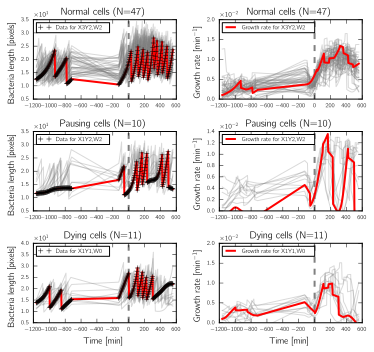
\includegraphics[scale=1]{./Fig/subcat_cells}
\caption{Subtypes of cells. Caption to write. Cutting the x axis might be a good idea because a third of the x-axis of each graph are "missing data".}
\label{fig:subcat_cells}
\end{figure}

\begin{figure}[p]
\centering
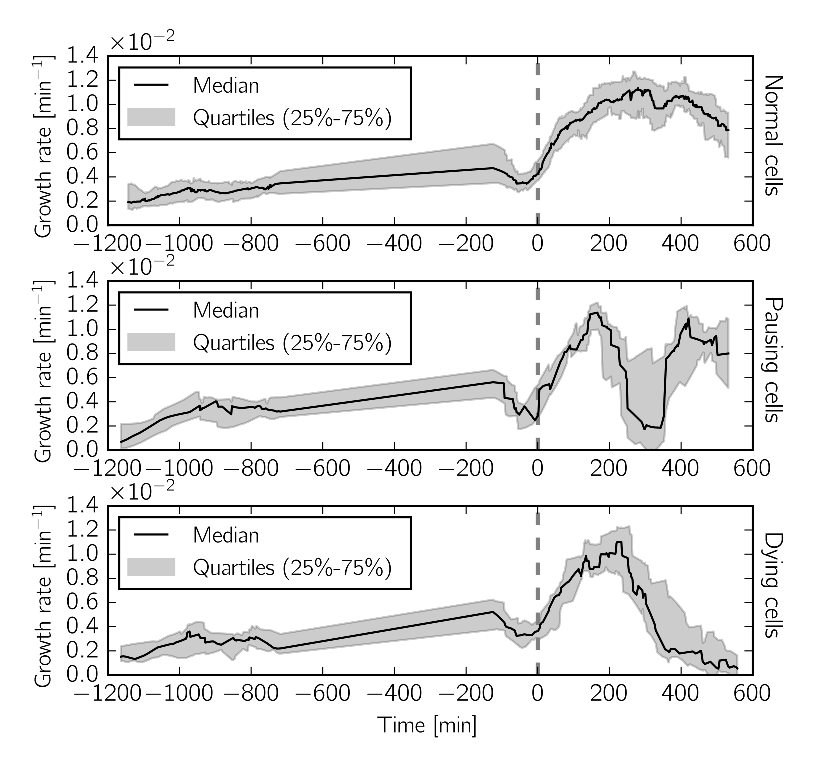
\includegraphics[scale=1]{./Fig/subcat_median}
\caption{Subtypes of cells, median. Caption to write.}
\label{fig:subcat_median}
\end{figure}